\documentclass[12pt, a4paper]{article}

%PACK------------------------------
\usepackage[utf8]{inputenc}
\usepackage[british, polish]{babel}
\usepackage{geometry}
\usepackage{gensymb} %pakiet symboli
\usepackage[upgreek, LGRgreek]{mathastext}
\usepackage{bm}
\usepackage{lipsum}
\usepackage{cite}
\usepackage{graphicx}
\usepackage{hyperref}
\usepackage{seqsplit}
\usepackage[monochrome]{xcolor}
\usepackage{mathptmx}
\usepackage{fontspec}
\usepackage{textcomp}

%SETTING---------------------------
%\defaultfontfeatures{LetterSpace=5}
\setmainfont{Times New Roman}
\setlength{\parindent}{0pt}
\setlength{\parskip}{0pt}
\linespread{1.25}
\geometry{left=2.54cm, right=2.54cm, top=2.54cm, bottom=2.54cm}
% \renewcommand{\thesection}{\arabic{section}.}
% \renewcommand{\thesubsection}{\thesection\arabic{subsection}.}
\newcommand*{\myfont}{\fontfamily{pcr}\selectfont}

%DOCUMENT--------------------------
\begin{document}
\begin{titlepage}
    \thispagestyle{empty}
    \begin{center}
    
        \textbf{\large Uniwersytet Jagielloński w Krakowie}
        
        \vspace{0.5cm}
        
        \textbf{\Large Wydział Biochemii, Biofizyki i Biotechnologii}
        
        \vspace{0.5cm}
        
        \begin{figure}[h]
            \centering
            \includegraphics[width=4cm]{figures/Herb_Uniwersytetu_Jagiellońskiego.svg.png}
            \label{fig:title}
        \end{figure}
        
        \vspace{0.5cm}

        \textbf{\huge Optymalizacja pomiarów napięcia w~układzie MFC z jednoczesną produkcją MlrA w komórkach \textit{Synechocystis sp.}}

        \vspace{2cm}

        {\Large Filip Stanisław Hajdyła}\\
        Nr albumu: 1164936

        \vspace{2cm}
        
        {\large Praca licencjacka z Biotechnologii}
        
        \vspace{0.5cm}
        
        {\large pod opieką dr hab. Dariusza Dzigi}
        
        \vspace{1cm}
        
        \textbf{\Large Pracownia Metabolomiki}
        
        \vspace{2cm}
        
        Kraków, 2022
        
    \end{center}
\end{titlepage}

\newpage
\thispagestyle{empty}
\begin{flushright}
    Dziękuję Panu Profesorowi Dariuszowi Dzidze\\
    oraz pozostałym członkom Pracowni Metabolomiki\\
    za cierpliwość, wyrozumiałość, cenne rady\\
    oraz pomoc w realizacji eksperymentów.
\end{flushright}
\vspace*{\fill}
\begin{flushleft}
    \textit{Non omnis moriar!}
\end{flushleft}


\newpage
\setcounter{page}{3}

\tableofcontents

\begin{abstract}
    \noindent
    \lipsum[1]
\end{abstract}

\vspace{0.5cm}

\begin{center}
    \rule{150pt}{0.4pt}
\end{center}

\vspace{0.5cm}

\begin{otherlanguage}{british}
    \begin{abstract}
        \noindent
        \lipsum[1]
    \end{abstract}
\end{otherlanguage}

\section{Wstęp teoretyczny}\label{sec:wstęp-teoretyczny}
\subsection{Historia \acrshort{mfc}}\label{subsec:historia}
\acrshort{mfc} (\textit{ang.} \acrlong{mfc}) to urządzenia umożliwiające
generowanie energii elektrycznej z wykorzystaniem mikroorganizmów.
Należą one do szerszej klasy urządzeń \acrshort{bes} (\textit{ang.}
\acrlong{bes})~\cite{Santoro2017}.
Pomysł wykorzystania mikroorganizmów do generowania elektryczności
przypisuje się Michaelowi Potterowi~\cite{Potter1911},
natomiast idea ,,elektryczności zwierząt'', a więc elektryczności
związanej z układami ożywionymi, sięga aż XVIII wieku~\cite{Santoro2017}.
Pomimo iż pracę Pottera uważa się za początek technologii \acrshort{mfc},
dopiero po ponad 50 latach od jej publikacji
znalazła ona praktyczne zastosowanie w oczyszczaniu i przetwarzaniu
odpadów ściekowych w prąd elektryczny podczas lotów kosmicznych
organizowanych przez \acrshort{nasa}~\cite{Slate2019}.

\subsection{Zastosowania \acrshort{mfc}}\label{subsec:zastosowania-mfc}

\begin{figure}[!b]
    \centering
    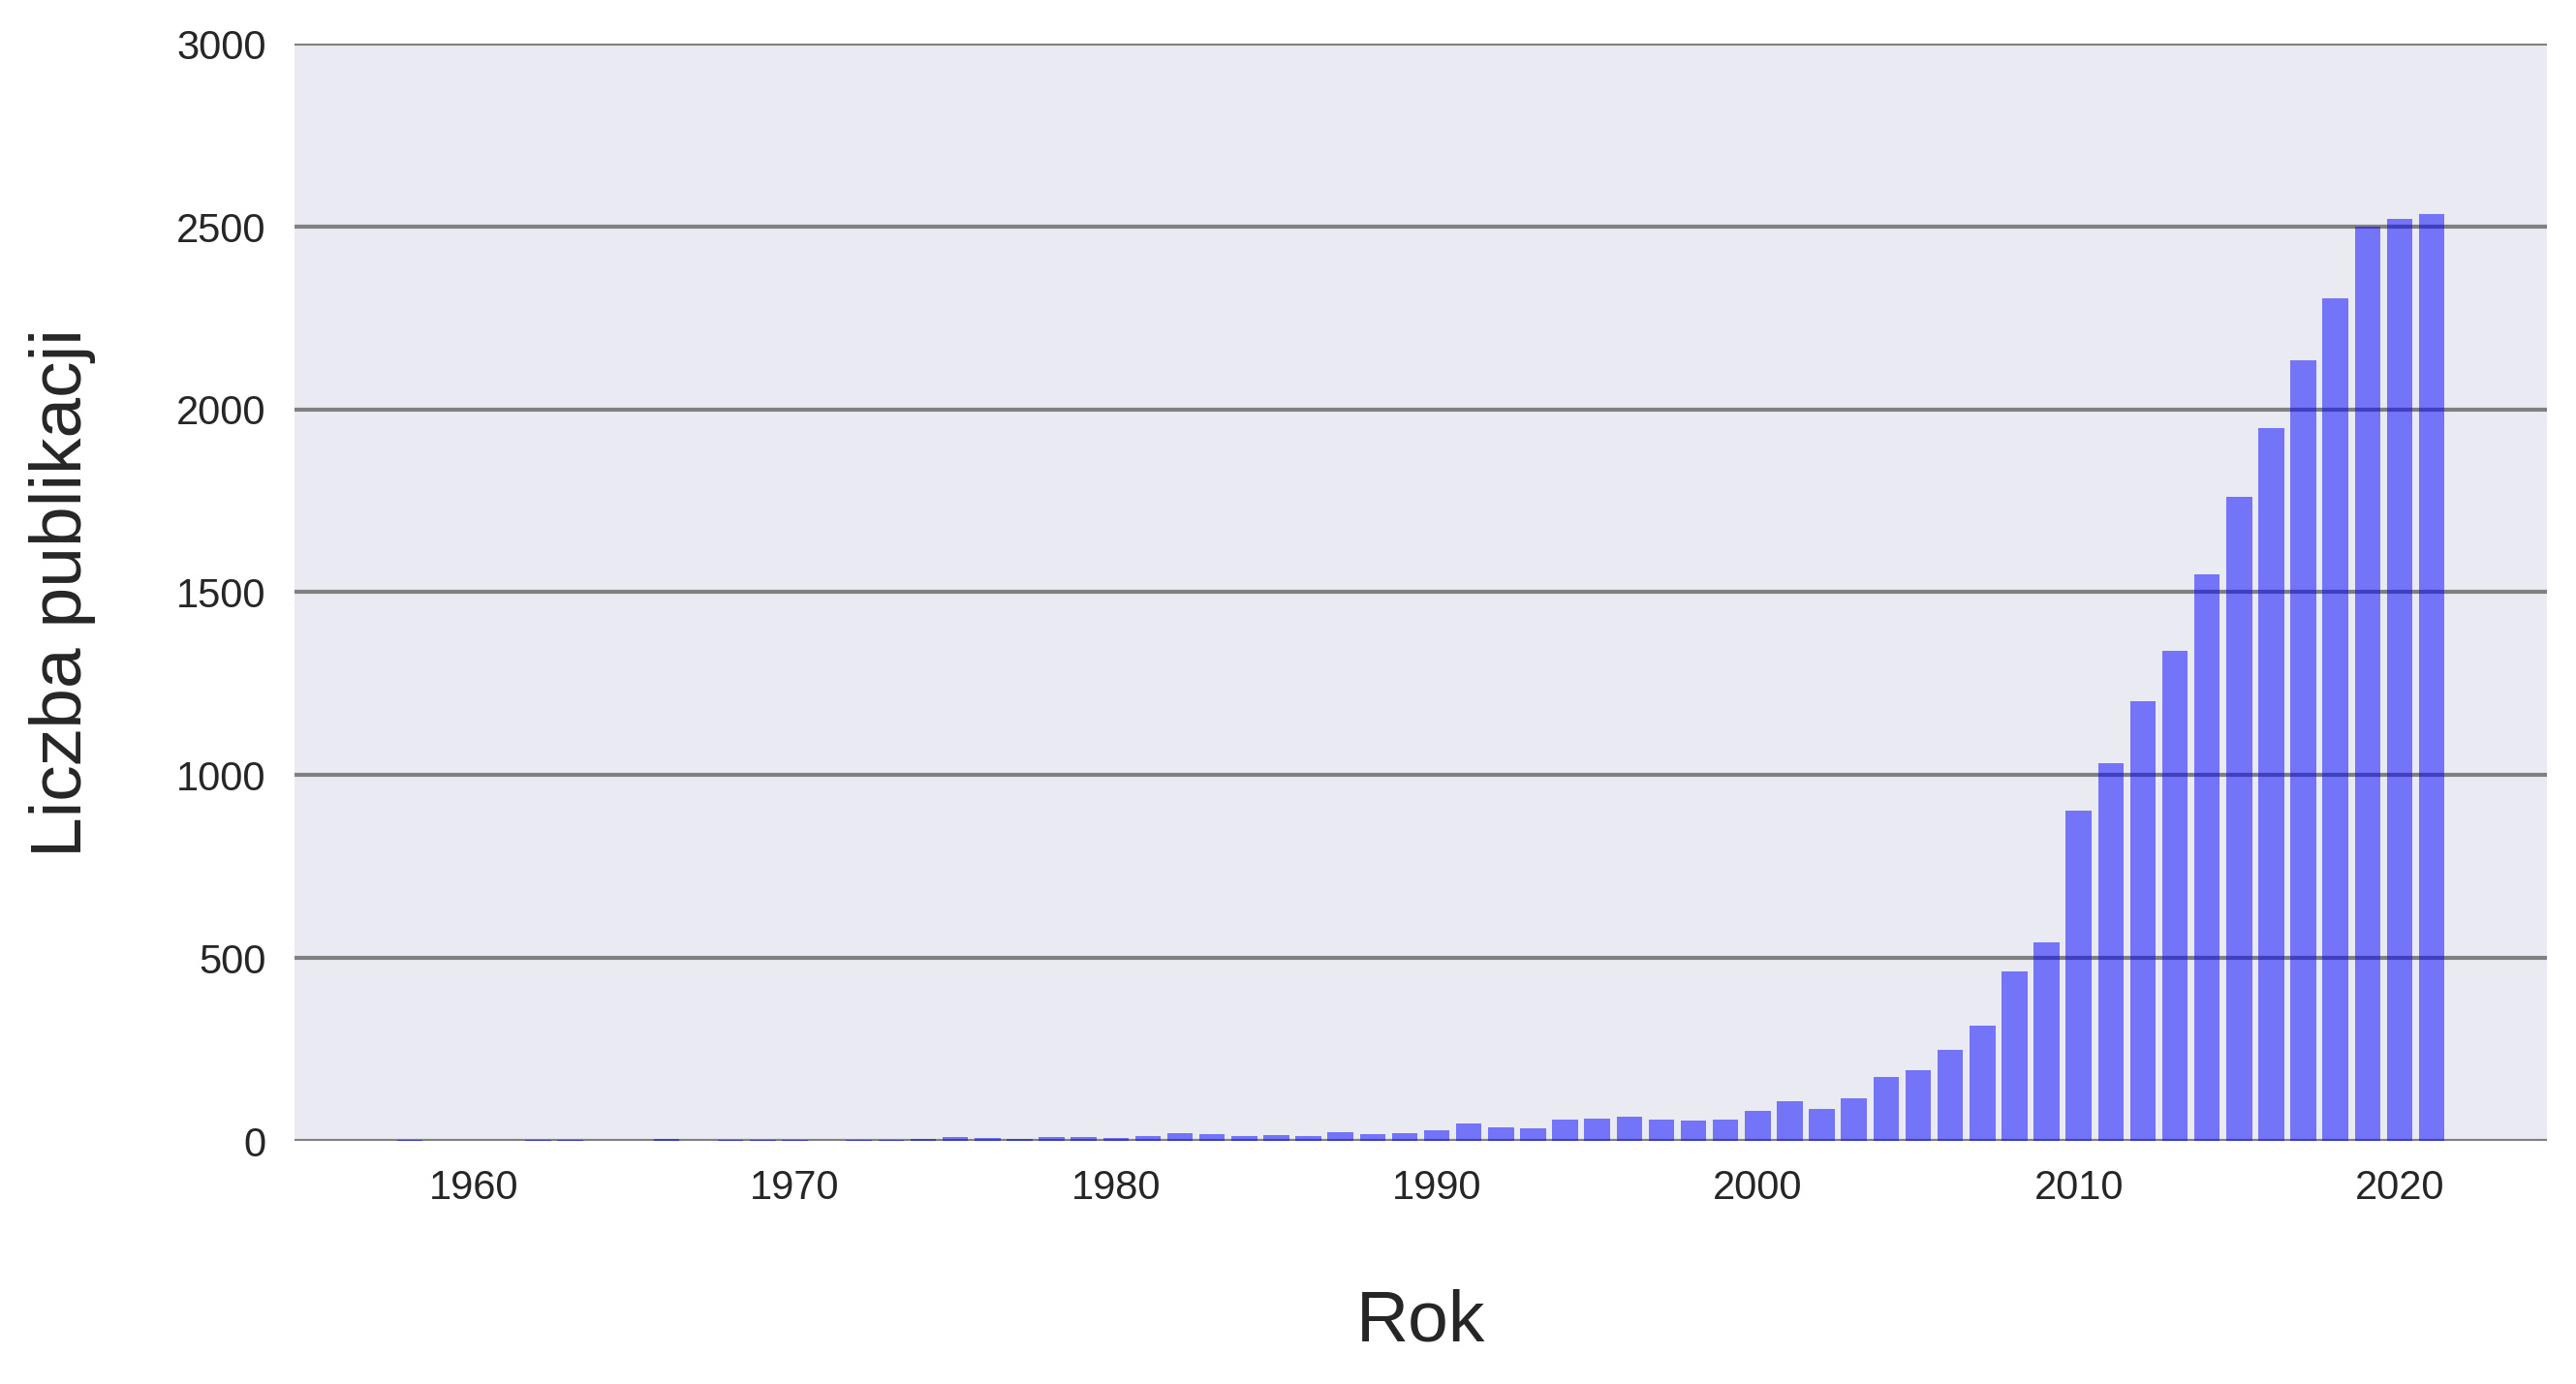
\includegraphics[width=12cm]{figures/publications}
    \caption{
        Liczba publikacji z ,,\acrshort{mfc}'' lub
        ,,\acrlong{mfc}'' w tytule w latach 1958--2021.
        (Dane pochodzą z serwisu \url{https://webofscience.com})
    }
    \label{fig:1}
\end{figure}

W ostatniej dekadzie zainteresowanie systemami \acrshort{bes},
a w szczególności \acrshort{mfc}, wzrosło diametralnie, co odzwierciedla wzrost
liczby związanych z nimi publikacji przedstawiony na rys.~\ref{fig:1}.
Pojawiające się publikacje związane z \acrshort{mfc}
dotyczą różnych aspektów tej technologii.
Wiele z nich dotyczy zrozumienia molekularnych podstaw
działania tych systemów~\cite{Slate2019, Bruce2006, Lovley2006}, inne
poruszają kwestie związane z ich konstrukcją i użyciem odpowiednich
materiałów do budowy elektrod i membran~\cite{Kaur2020, Daud2015},
a jeszcze inne skupiają się na bardzo istotnych
aspektach ekonomicznych~\cite{Trapero2017}.
Wysokie zainteresowanie technologią \acrshort{mfc} w ostatnich latach wynika
z potencjału do wykorzystania ich w celu jednoczesnego oczyszczania
wód ściekowych, generowania energii elektrycznej oraz produkcji cennej biomasy,
która mogłaby następnie zostać wykorzystana w biorafineriach do produkcji
biopaliw, biopolimerów i biochemikaliów.
Niewątpliwymi zaletami tych systemów są również ich długi czas działania
bez konieczności konserwacji i obsługi~\cite{Habermann1991}
oraz niewymagające warunki operacyjne~\cite{Slate2019}.
Obecne systemy oczyszczania ścieków wykorzystujące osad czynny
zużywają od 0.3 do 0.6 kWh m\textsuperscript{-3} co w skali globalnej
przekłada się na 4 \% całkowitego zużycia energii~\cite{AlSayed2020}.
Wszystkie ww.\ zalety systemów \acrshort{mfc} sprawiają natomiast, że mogłyby one
być częściowym rozwiązaniem problemu nadmiernej akumulacji odpadów,
umożliwiając ich energetycznie korzystną biokonwersję.
Obecnie uważa się, że systemy te nie są w stanie całkowicie zastąpić
tradycyjnych oczyszczalni ścieków, ale mogłyby służyć
jako jeden z komponentów nowoczesnych oczyszczalni połączonych
z biorafineriami.

\subsection{Podstawy molekularne działania \acrshort{amfc}}\label{subsec:podstawy-molekularne}
W systemach \acrshort{amfc} (\acrlong{amfc}), do generowania elektryczności, wykorzystuje się
utleniająco-redukujący charakter reakcji metabolicznych
przeprowadzanych przez mikroorganizmy, które możemy podzielić
na rezydujące na powierzchni anody elektrogeny (uwalniające na nią
elektrony) oraz zasiedlające katodę elektrotrofy
(pobierające i wykorzystujące elektrony)~\cite{AlSayed2020}.
Elektrogeny przeprowadzają procesy oddychania beztlenowego,
utleniając znajdujące się w pożywce związki organiczne oraz
wykorzystując anodę jako ostateczny akceptor elektronów.
Przykładem takiego procesu może być utlenianie octanu:
\begin{equation}
    \label{eq:1}
    \mathrm{CH_3 COO^- + 4H_2 O \rightarrow 2HCO_3^- + 9H^+ + 8e^-}
\end{equation}
Zdolność do transferu elektronów na powierzchnię metali (lub
innych przewodników) wynika z~naturalnego przystosowania tych
organizmów do życia na powierzchni rud metali i wykorzystania
ich jako ostateczny akceptor elektronów.
Transfer elektronów na elektrodę może zachodzić na różne
sposoby~\cite{Santoro2017}:

\begin{enumerate}
    \item Transport bezpośredni (z wykorzystaniem cytochromu c);
    \item Transport przez nano-przewody;
    \item Transport za pośrednictwem mediatorów redox;
\end{enumerate}

Choć nie poznano jeszcze dokładnie molekularnych mechanizmów
transferu elektronów, wiadomo, że najwolniejszym oraz
niekorzystnym z technologicznego punktu widzenia sposobem jest
transport za pośrednictwem mediatorów redox, gdyż jest on znacznie
ograniczony szybkością dyfuzji.
Do najbardziej efektywnych elektrogenów należą
\textit{Geobacter sulfurreducens}, \textit{Shwanella oneidensis}
oraz \textit{Rhodobacter sphaeroides}.
Elektrotrofy są z kolei organizmami pobierającymi elektrony
z powierzchni katody (za pośrednictwem mediatorów redox)
i redukującymi CO\textsubscript{2}, lub organizmami przeprowadzającymi fotosyntezę
oksygeniczną~\cite{Santoro2017, Reddy2019}.
Uwolniony w wyniku procesu fotosyntezy tlen jest następnie wykorzystywany
do utylizacji elektronów w reakcji redukcji tlenu do wody:
\begin{equation}
    \label{eq:2}
    \mathrm{O_2 + 2H^+ + 2e^- \rightarrow H_2 O}
\end{equation}
Użycie organizmów zapewniających wysokie tempo zużycia elektronów np.
intensywnie fotosyntetyzujących alg, takich jak \textit{Chlorella vulgaris},
lub cyjanobakterii z rodzaju \textit{Synechocystis} pozwala na efektywne
zapewnienie odpowiednich ilości tlenu w komorze katodowej bez
konieczności jej mechanicznego napowietrzania, co pozwala dodatkowo
zmniejszyć koszty operacyjne~\cite{Reddy2019}.
Należy jednak pamiętać, aby zapewnić odpowiednie warunki
organizmom bytującym w komorze z katodą.

\subsection{Cel pracy}\label{subsec:badania}
W niniejszej pracy przeprowadzono wstępne badania wzrostu organizmów
elektrogenicznych i elektrotroficznych
w środowisku o wysokim zanieczyszczeniu związkami
organicznymi, z jednoczesnym pomiarem aktywności mikrocystynazy
\acrshort{mlra}~\cite{Dexter2018, Dexter2021} w komórkach elektrotrofów
(\textit{Synechocystis sp.} PCC 6803),
oraz na optymalizacji pomiarów napięcia prądu elektrycznego generowanego
podczas wzrostu i metabolizmu tych mikroorganizmów.
Praca Pani Konstancji Gałat dowiodła, że w przypadku
hodowli z użyciem rozcieńczonych ścieków komunalnych (\acrshort{ww})
jako pożywki, największą ekspresję \acrshort{mlra} wykazuje szczep
\textit{Synechocystis sp.} PCC 6803 McCormick 7 rosnący na pożywce
z dodatkiem \acrshort{ww}2 (\ref{subsec:odczynniki})~\cite{Galat2022},
dlatego w niżej opisanych badaniach użyty został właśnie ten szczep,
a do jego kultywacji wykorzystano ww.\ substrat.

\section{Metody}\label{sec:metody}

\subsection{metoda 1}
\lipsum[2]
\subsection{eksperyment uno}
\lipsum[3-5]

\section{Analiza Danych}\label{sec:analiza-danych}
\subsection{dane}
\lipsum[2-4]
\subsection{więcej danych}
\lipsum[2-4]
\subsection{jeszcze więcej zasranych danych}
\lipsum[2-4]

\begin{otherlanguage}{polish}
    \newpage
    \thispagestyle{empty}
    \bibliographystyle{plain}
    \bibliography{main}
\end{otherlanguage}



\end{document}


